The domain is a unit square. Free slip 
boundary conditions are prescribed on all sides.
The resolution is fixed to 64x64 $Q_1 \times P_0$ elements. 
The flow is isoviscous and the buyancy force is given by 
\begin{eqnarray}
f_x &=& 0 \\
f_y &=& \rho \alpha T(x,y) 
\end{eqnarray}
with 
\[
T(x,y) = \cos(kx) \delta(y-y_0)
\]
where $k=2\pi/\lambda$ and $\lambda$ is a wavelength, 
and $y_0$ represents the location of the buoyancy.

One can prove \cite{zhgh93} and refs. therein that 
there is an analytic solution of the surface stress 
$\sigma_{zz}$:
\[
\frac{\sigma_{yy}}{\rho \alpha g} =
\frac{\cos (kx)}{\sinh^2(k)}
\left[
k(1-y_0)\sinh(k) \cosh(ky_0)-k \sinh(k(1-y_0))
+\sinh(k) \sinh(ky_0)
\right]
\]

We set $\lambda=1$ and explore $y_0 = \frac{63}{64},\frac{62}{64},\frac{59}{64}$.
Zhong et al. report for measurements at $x=0$:

\begin{center}
\begin{tabular}{llll}
\hline
Method             & $y_0=63/64$ & $y_0=62/64$ &  $y_0=59/64$ \\ 
\hline
\hline
Analytic solution  & 0.995476    & 0.983053    &  0.912506 \\
Pressure smoothing & 1.15974     & 1.06498     &  0.911109 \\
CBF                & 0.994236    & 0.982116    &  0.912157 \\
\hline
\end{tabular}
\end{center}


We are then interested in numerically computing this quantity:
\[
\sigma_{yy} = -p + 2 \eta \dot{\epsilon}_{yy}
\]
and we start with the trivial measurement in the middle of the elements 
forming the top row of the mesh. 

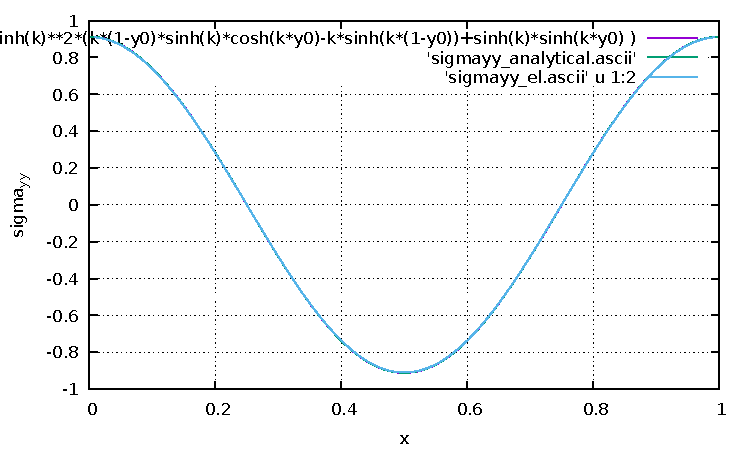
\includegraphics[width=12cm]{python_codes/fieldstone_27/results/elemental/sigmazz.pdf}






\fbox{
\parbox{10cm}{{\bf features}
\begin{itemize}
\item $Q_1\times P_0$ element \index{$Q_1 \times P_0$}
\item incompressible flow \index{incompressible flow}
\item mixed formulation \index{mixed formulation}
\item isothermal \index{isothermal}
\item isoviscous \index{isoviscous}
\item analytical solution \index{analytical solution}
\item pressure smoothing \index{pressure smoothing} 
\item consistent boundary flux \index{CBF}
\end{itemize}
}}

